\documentclass[a4paper,12pt]{book}


\usepackage[english]{babel}
\usepackage{blindtext}

%\usepackage[scaled=.92]{helvet}

\usepackage{microtype}
\usepackage{graphicx}
\usepackage{svg}
\usepackage{float}

\usepackage{algorithm}
\usepackage{algorithmicx}
\usepackage{caption}
\usepackage{wrapfig}
\usepackage{subfigure}
\usepackage{enumitem} 
\usepackage{amsmath, bm}
\usepackage{index}
\usepackage{algpseudocode}

%\usepackage{paralist}
%\usepackage{parskip}
%\usepackage[doublespacing]{setspace}
% \usepackage[latin1]{inputenc}
\makeindex


\graphicspath{ {./resources/infografika} }
\svgpath{resources/infografika/}



\begin{document}
\title{\Large{\textbf{Test}}}
\author{Adamofus}
\date{December 21, 2022}
\maketitle
\let\cleardoublepage\clearpage
\tableofcontents

	
\pagenumbering{roman}
\setcounter{page}{2}



\chapter{Projekce scény}
Projekcí scény je v této práci myšleno perspektivní vidění.
Paprsek jdoucí od promítaného bodu do oka pozorovatele se promítá na určenou rovinu v prostoru, tz. tvoří průnik s touto rovinou. Výsledný bod je přenesený na 2D soustavu souřadnou v této rovině.



\section{Stínění objektů v 3D}
\section{Zoom}




\chapter{Rasterizace}


Rasterizace je proces převodu vektorově definované grafiky do tzv. rastru, tedy mřížky skládající se z bodů (pixelů).
Takový rastr je základem obrazového výstupu na digitálních zařízení.
V následujícíh kapitolách jsou představeny algoritmy rasterizace 2 objektů: úsečky a kruhu.
Samostatná kapitola je pak věnovaná rasterizaci Beziérových křivek.


\section{Úsečka}



Převedení vstupu\\
Úsečka je část přímky definovaná dvěma body: $b_1$ a $b_2$.
Pro následující algoritmy platí, že souřadnice $x$ bodu $b_1$ je menší než $x$ bodu $b_2$, aby se mohly algoritmy posouvat o jeden dílek doprava, tj $x+1$.
Směrnice úsečky je $a = dy/dx$. 
Počítá se s vstupem $a\subset<0;1>$, takže úsečka svírá s osou $x$ úhel $0-45$ a $b_2$ je v 1. kvadrantu. Opět pro omezení na jedinou podmínku, zda je potřeba $y$ zvětšit či nikoli.


Tyto nároky umožňují zvolit efektivní algoritmus, ale současně vyžadují převod vstupu a výsledných souřadnic.\\

\begin{figure}[H]
  \centering
  \includesvg{fig1}
  \caption{Převod souřadnic podle směrnice úsečky.}
\end{figure}

%\includesvg[width=0.6\columnwidth](fg1.svg)



DDA\\
DDA využívá zaokrouhlované hodnoty $n*a$ pro výpočet $y_{new}$, je to prostý přístup. Současně ale zbytečně používá funkci zaokrouhlování či přetypování, kterou lze pro optimalizaci nahradit podmínkou s použitím proměnné,
protože jsou pouze 2 možnosti pro $y_{next}$: $y_{next} = y$, nebo $y_{next} = y+1$.

Proměnnou vyjadřuje $error(n)=((n*a)\mod1)-1/2$, kde $n$ je krok iterace, takže $error(0) = -1/2$.
Pokud platí zmíněná podmínka $error(n) >= 0$, platí současně $y_{next}=y+1$ a $error(n+1) = error(n) + a - 1$, jinak platí $error(n+1) = error(n) + a$.


Bresenhamův algoritmus\\
Další optimalizací je zbavení se desetinné čárky (tzv. float point number).
Představme si $error(n) = 2*dx*error(n)$. Jsou 2 možnosti:


$error(n+1)=error(n)+2*dy$\\
$error(n+1)=error(n)+2*dy-2*dx$

Nerovnice podmínky se nemění, protože po vynásobení pravé strany $2*dx$: $error(n+1)>=0*2*dx$ zůstává stejná.
Tím jsme se zbavili nutnosti použití desetinné čárky.




% tloustka cary, prostor, zdroje, infografika


\begin{algorithmic}
\State $x \gets x_1$
\State $y \gets y_1$
\While{$x<=x_2$}
\\vykresli bod[x,y]
\State $x \gets x + 1$
\State $error \gets error + 2d_y$
\If{error $\geq 0$}
    \State $y \gets y + 1$
    \State $error \gets error - 2d_x$
\EndIf 
\EndWhile
\end{algorithmic}





\section{Zrcadlení}

Zrcadlení je často využívaná operace, například pro rasterizaci kružnice.
Využívá bod $B$ a vektor $\vec{v}$, přes který $B$ zrcadlíme. Výstupem je zrcadlený bod $B_{z}$.
Platí, že vektor $\overrightarrow{BB_{z}}$ je kolmý na $\vec{v}$ a jeho délka je dvojnásobná vzdálenosti $B$ od $\vec{v}$.


$\frac{1}{2} \overrightarrow{BB_{z}} = (k*x+P_x;k*y+P_y)-(b_x;b_y)$, skalární součin tedy:
\\$(k*x+P_x-b_x;k*y+P_y-b_y)*(x;y)=0$.
\\Úpravou rovnice vyjde $k = -\frac{x(B_x-P_x)+y(B_y-P_y)}{x^2+y^2}$, bod získám:
$B_z = 2(k*\vec{v}+P)-B) = \bm{(2(k*x+P_x)-B_x;2(k*y+P_y)-B_y)}$



%$$




\section{Kruh} % Obdelník, trojúhelník, kružnice, elipsa, kvádr a koule

Pro kužnici rovněž existuje Bresenhamův algoritmus. Algoritmus vykreslí $1/8$ kružnice. V podmínce je tedy ze znalosti přímky svírající s osou $x$ 45 stupnu: $x>=y$. K vykreslení této části víme, že iterativně zvětšujeme $y$. $x$ dekrementujeme, pokud je hodnota $d$ kladná, tj. zajímají nás pouze 2 pixely. %infografika
Pro vykreslení celku stačí díky symetrii kružnice tuto část 3x zrcadlit.




\begin{algorithmic}
\State $d \gets x^2 + y^2 - r^2$
\State $x \gets r$
\State $y \gets 0$
\State $d \gets 0$
\While{$x>=y$}
\\vykresli bod[x,y]
\State $y \gets y + 1$
\State $d \gets d + d_y$
\If{$d \geq 0$}
    \State $x \gets x - 1$
    \State $d \gets d - d_x$
\EndIf 
\EndWhile
\end{algorithmic}

Jiný algoritmus se může zakládat na výběru z 3 sousedících pixelů podle toho, který je nejblíž středu. Takové řešení je ale neefektivní, implementací se zde nezabývám.






\section{Ostatní}

\section{Bezierova křivka}

\section{Vyplňování} % vyplňování jednoduchých tvarů a polygonů


Řádkovací metoda


\begin{figure}[H]
  \centering
  \includesvg[width=1\textwidth]{fig2}
  \caption{Vyplňování řádkováním ze shora dolů. Červené vrcholy nevedou na žádnou další úsečku, zelené vedou na 2 úsečky a modré vedou na druhou přiléhající úsečku.}
\end{figure}



\begin{algorithm}
\caption{Řádkovací metoda}
\begin{algorithmic}


\Function{solve}{$x$, $y$}
\State $row \gets \text{maxY(points)}$
\State $points[], init[],arr\_a[],lines\_points[] \gets []$
%cecko rozumi points[-1], ale musí se ošetřit případ point[len(points)+1], takže se přidá první bod na konec
\State $points[] \gets [points[...],points[0]]$
\For{$i = 0$; $i = \text{len(init)}$; $i++$}
  \For{$b\_idx = 1$; $b\_idx < \text{len(init[i])}$; $b\_idx++$}
   \State $b\_val \gets $init[$i][$b\_idx]
    \For{$b\_tmp = 0$; $b\_tmp < \text{len(tmp)}$; $b\_tmp++$}
	\If{b\_val$=tmp[b\_tmp]$}
	 \State $found \gets \text{true}$
	  %je `y' dalšího bodu < `y' bodu b_val?
	  \If{$y(points[b\_val-1])<y(points[b\_val])$}
	  	 %=>tmp[b_tmp]=idx dalšího bodu
		 %=>arr_a[b_tmp]='dx/dy' mezi body b_val a dalšího bodu
	  	\State $tmp[b\_tmp] \gets b\_val-1$
	  	\State $arr\_a[b\_tmp] \gets get\_dx(b\_val,b\_val-1)$
	\ElsIf{$y(points[b\_val+1])<y(points[b\_val])$}
	  	\State $tmp[b\_tmp] \gets b\_val+1$
	  	\State $arr\_a[b\_tmp] \gets get\_dx(b\_val,b\_val+1)$
	%není=>smaž tmp[b_tmp],arr_a[b_tmp],lines_points[b_tmp]
	\ElsIf{$y(points[b\_val+1])==y(points[b\_val]) || y(points[b\_val+1])=y(points[b\_val])$}
		\State \text{remove(tmp[b\_tmp],arr\_a[b\_tmp],lines\_points[b\_tmp])}
	\Else
		\State \text{remove(tmp[b\_tmp],arr\_a[b\_tmp],lines\_points[b\_tmp])}
		\State \text{remove(tmp[b\_tmp],arr\_a[b\_tmp],lines\_points[b\_tmp])}
	  \EndIf
		 \State \text{break}
	\EndIf
\EndFor
\If{$!found$}
		\\\Comment{jsou zde 2 nové (neuvažované) úsečky. každá s tímto bodem}
%pridej `a' obou useckech v kterych je tento bod a pridej za pole, proste pridej do danych poli
	
	  	
	  	\State $tmp.add(b\_val+1,b\_val-1)$
	  	\State $arr\_a.add(get\_dx(b\_val,b\_val+1),get\_dx(b\_val,b\_val-1))$
	  	
	  	\State $new\_x \gets x(points[b\_val])$
	  	\State $lines\_poins.add(new\_x, new\_x)$
\EndIf
\EndFor


\For{$y = 0$; $y < \text{init[i][0]}$; $y++$}
	\State $row \gets row-1$

\For{$k = 0$; $k < \text{len(lines\_points)}$; $k+=2$}
	\State $A_x \gets lines\_points[k] \gets lines\_points[k] + arr\_a[k]$
	\State $B_x \gets lines\_points[k+1] \gets lines\_points[k+1] + arr\_a[k+1]$
	\For{$x = A_x$; $x < B_x$; $x++$}
	\\\Comment{přidej bod [x,row]}
	\EndFor	
\EndFor


\EndFor


\EndFor
\EndFunction

\Function{get\_dx}{$A\_idx$, $B\_idx$}
    \State $pointA \gets points[A\_idx]$
    \State $pointB \gets points[B\_idx]$
    \State \textbf{return} $\frac{x(pointB)-x(pointA)}{y(pointB)-y(pointA)}$
\EndFunction


\end{algorithmic}
\end{algorithm}








Vyplňování rozbitím do trojúhelníků

Metoda rozbije libovolný konkávní polygon do trojúhelníků, které už stačí vyplnit úspornou metodou vyplňování trojúhelníka.
Algoritmus omezuju na vstup konkávního polygonu, protože konvexní polygon vyžaduje odlišný přístup - zejména ověření úhlu, který hrany svírají (konkávní/konvexní?). Podoba algoritmu by v intencích původní myšlenky nutně zahrnovala komplexnější přístup.




%jak se vyplňuje trojúhelník?

\begin{algorithm}
\ContinuedFloat
\caption{Solve}
\begin{algorithmic}
\caption{Vyplňování rozbitím do trojúhelníků}
\State $points[] \gets []$

\Function{solve}{}
\State $nB \gets len(points)$
\State $b\_i \gets 0$
\State $C \gets 0$

\While{$nB > 3$}

\State $A \gets C$

\While{$!arr[(++b\_i)\%len(points)]$}
\EndWhile

\State $B \gets b\_i$

\State $arr[B] \gets false$

\While{$!arr[(++b\_i)\%len(points)]$}
\EndWhile

\State $C \gets b\_i$

\State $nB \gets nB-1$

\State $fillTriangle(A,B,C)$

\EndWhile

%zbývá vyplnit poslední trojúhelník. body A a C jsou uloženy v proměných, ale zbývající 3. bod B není známý..ten bude dál ve směru procházení od C
\State $B \gets C$
\While{$!arr[(++C\%len(points))]$}
\EndWhile
\State $fillTriangle(A,B,C)$
\EndFunction

\Function{get\_dx}{$A\_idx$, $B\_idx$}
    \State $pointA \gets points[A\_idx]$
    \State $pointB \gets points[B\_idx]$
    \State \textbf{return} $\frac{x(pointB)-x(pointA)}{y(pointB)-y(pointA)}$
\EndFunction
\end{algorithmic}
\end{algorithm}

\begin{algorithm}
\begin{algorithmic}
\ContinuedFloat
\caption{Vyplnění trojúhelníka}
\Function{fillTriangle}{A,B,C}

\State $a \gets minY(A,B,C)$
\State $b \gets middleY(A,B,C)$
\State $c \gets maxY(A,B,C)$

\State $a_1 \gets get\_dx(B,C)$ %C-B
\State $a_2 \gets get\_dx(A,B)$ %B-A
\State $a_3 \gets get\_dx(A,C)$ %C-A

\State $fP \gets x(C)$
\State $sP \gets x(C)$

\State $y \gets y(C)$

\For{$y\_p = y(c)$; $y < y(b)$; $y--$}
	% a1-a3
	\State $fP \gets fP+a_1$
	\State $sP \gets sP+a_3$
	
	\State $x \gets fP$
	\While{$++x<sP$}
	\\\Comment{přidej bod [x,y\_p]}
	\EndWhile	
\EndFor



\For{$y\_p = y(c)$; $y < y(b)$; $y--$}
	% a2-a3
	\State $fP \gets fP+a_2$
	\State $sP \gets sP+a_3$

	
\EndFor



\EndFunction





\end{algorithmic}
\end{algorithm}





Flood fill




\chapter{Analýza}
\section{Bod v polygonu}
Pokud je polygon otevřený, žádný bod by správně neměl ležet v polygonu. V takovém případě stačí buď ověřit, zda je polygon úplný a neprůnikuje se. Prakticky v programu k tomu nedojde, přesto je možné obě věci obejít tv. winding číslem. Bod leží mimo polygon, pokud je 0, jinak leží uvnitř.


\section{Konvexní/konkávní}
 \begin{figure}[H]
  \centering
  \includesvg[width=1\textwidth]{fig6}
  \caption{Identifikace konvexního/konkávního polygonu}
\end{figure}
\section{Detekce kolize}
\section{Oblasti průniku dvou objektů a průřez}

Pro jasnost uvádím, že polygon A je polygon, který průnikuje polygon B. Výsledný průnik (polygon) označuju C.

Sutherland–Hodgman algoritmus


Pokud pomyslně prodloužíme hrany A, můžeme dělit strany této hrany na stranu, kde se nachází zbytek A a tedy i na stranu, v které se nenachází ani jeden vrchol A. Jakýkoli bod na  druhé straně polygonu není určitě uvnitř A, takže ho nepoužijeme pro C. Pokud je tomu naopak, bod necháme. Postup se totiž opakuje pro každou další stranu A, tz. že na konci zbydou pouze body (vrcholy B), které uvnitř A leží. Mezi body se navíc při procházení zjištuje, jestli průnikují B, v takovém případě se přidává navíc i bod jako průsečík hran. Algoritmus je omezen pouze na konvexní A. V opačném případě nemusí fungovat koncept (nebo by nutně vyžadoval zbytečně náročnou modifikaci), protože bychom mohli vyloučit body, které jinak v polygonu leží. Současně B je nutně konvexní. V opačném případě může dojít k překrytí (tz. overlaping) hran C - v tomto případě by vzniklo výsledků víc jako víc polygonů/samostatných průnikových oblastí. Problém řeší Vattiho algoritmus, který zaznamenává body při vstupu B do A končí při výstupu B z A. Potom přidá body na A mezi $I_{vstup}$ a $I_{vystup}$ ve směru procházení, kterým procházíme vrcholy B.

%grafika - oba algoritmy
%algoritmus - vatti
%dalsi - 
%Weiler–Atherton clipping algoritmus
%Greiner–Hormann clipping algorithm



\begin{figure}[H]
  \centering
  \includesvg[width=1\textwidth]{fig7}
  \caption{Vatti clipping algoritmus}
\end{figure}



\section{Obsah polygonu}

Obsah polygonu si lze
$S_i = (x_1-x_2)*\frac{y_1+y_2}{2}$

\begin{figure}[H]
  \centering
  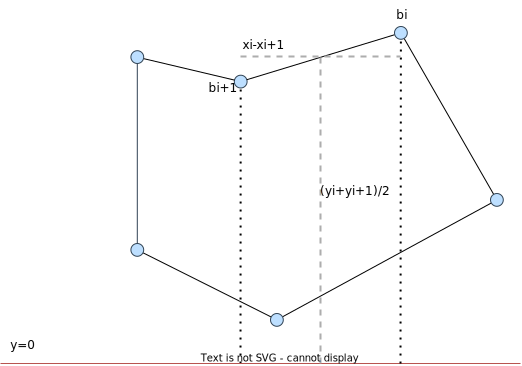
\includegraphics[width=1\textwidth]{fig8.png}
  \caption{Vatti clipping algoritmus}
\end{figure}


\section{Je A v B?}




\chapter{Rotace}


Otáčet bod vůči středu soustavy souřadné je jako nanášet ho na otočenou soustavu souřadnou, tedy násobit vektory udávájící osy $x$, $y$, atd. takové soustavy.
Tyto vektory mají délku 1. Lze zapsat takto:

$p_n = \begin{pmatrix}
X_1 & Y_1 \\
X_2 & Y_2
\end{pmatrix}\vec{p}$\\


\section{2D}

Otočené souřadnice můžeme vyjádřit takto:


$X_1 = \cos(-\alpha) = \cos(\alpha)\\
X_2 = \sin(2\pi-\alpha) = -\sin(\alpha)\\
Y_1 = \cos(\pi/2 - \alpha) = \sin(\alpha)\\
Y_2 = \sin(\pi/2 - \alpha) = \cos(-\alpha) = \cos(\alpha)
$\\



$\begin{pmatrix}
\cos(\alpha) & \sin(\alpha)\\
-\sin(\alpha) & \cos(\alpha)
\end{pmatrix}\begin{pmatrix}x\\y\end{pmatrix}$



\section{3D}

Rotace bodu vůči ose Z ve směru hodinových ručiček:\\
$\begin{pmatrix}
\cos(\alpha) & \sin(\alpha) & 0\\
-\sin(\alpha) & \cos(\alpha) & 0\\
0 & 0 & 1
\end{pmatrix}\begin{pmatrix}x\\y\\z\end{pmatrix}$\\

Rotace bodu vůči zvolené ose:\\

Máme vstup osu $o$ a úhel $\alpha$. 

Mějme 2 soustavy souřadné $A$ a $B$ popsané jednotkovými vektory. Přitom $A$ je naše výchozí, na které vykreslujeme:

$\begin{pmatrix}
1 & 0 & 0\\
0 & 1 & 0\\
0 & 0 & 1
\end{pmatrix}$\\

Matice B má tvar:

$\begin{pmatrix}
a_x& b_x& o_x\\
a_y & b_y& o_y\\
a_z & b_z & o_z
\end{pmatrix}$\\

3. řádek $B$ tvoří souřadnice osy $o$, takže 3. souřadnice $p_b$ je právě vzhledem k $o$.

Čili je z následující rovnice zaručeno, že získáme přesně takový bod $p_b$, kde jeho 3. souřadnice je vzhledem k $o$. To potřebujeme, protože jsme zvolili matici
rotace podle osy Z (respektive 3. osy...), kterou chceme bod násobit. Takže tato souřadnice bodu v $B$ po rotaci bude stejná.

Z rovnice $p_a = p_b B$ vyjádříme tedy $p_b$ vynasobením $B^{-1}$: $p_b = p_a B^{-1}$\\ %!


Zbývající vektory $a$ a $b$ v $B$ musí být jednotkové a vzájemně kolmé. takový $a$ dostaneme třeba ignorováním $z$ a přehozením souřadnic následovně: $\vec{a} = \{-y, x, 0\}$, kde $x$ a $y$ jsou souřadnice $o$. $b$ je už jen vektorovým součinem $a$ a $b$.

To je tedy převod relativních souřadnic ze soustavy $A$ do soustavy $B$.

% Prakticky nesejde na určení výchozího směru rotace.



Rotace probíhá následovně:\\

Vstup: osa otáčení $o$, úhel $\alpha$

\begin{enumerate}[label=\arabic*, font=\bfseries] % nummbered list
	\item převedeme souřadnice z A do B
	\item zrotujeme (například přes matici 1.1, tj. vůči 3. ose)
	\item vykreslujeme v A, takže převedeme z B do A
\end{enumerate}



\section{Posunutí středu a osy otáčení}

Pro posunutý střed v 2D platí, že vektor $\vec{XS}$, kde $S$ je střed a $X$ bod, má fakticky souřadnice bodu $\vec{p}$. K výpočtu stačí potom přičíst $S$.\\

Stejně u posunuté osy v 3D, je takový vektor vlastně bod $p_a$
V praxi, grafickém editoru, můžeme osu určit typicky dvěma body. A ten jeden z nich (třeba pro intuici první určený) je totiž tento střed $S$. Nakonec stačí opět přičíst $S$.


\chapter{Generování tvarů a fraktály}


\begin{figure}[H]
  \centering
  \subfigure[Caption for first figure]{\includesvg[width=0.3\textwidth]{fig3}}
  \hfill
  \subfigure[Caption for second figure]{\includesvg[width=0.3\textwidth]{fig4}}
    \hfill
  \subfigure[Caption for second figure]{\includesvg[width=0.3\textwidth]{fig5}}
  \caption{Schémata generování polygonu}
  \centering
\end{figure}
 



 



\end{document}



